\documentclass{beamer}
%\documentclass[handout,t]{beamer}

\batchmode
% \usepackage{pgfpages}
% \pgfpagesuselayout{4 on 1}[letterpaper,landscape,border shrink=5mm]

\usepackage{ctex,amsmath,amssymb,enumerate,epsfig,bbm,calc,color,ifthen,capt-of}
\usepackage{url} 
\usepackage{hyperref} 
\usepackage{geometry}
\usepackage{amsmath}
\usepackage{array}

\usetheme{Berlin}
%\usecolortheme{mit}

\title{媒体云转码的演进:\\\Small{MapReduce、DASH与稳定婚姻}}
\author{Alan Zhuang\\
\href{mailto:cheedoong@acm.org}{\nolinkurl{cheedoong@acm.org}}\\
}
\date{\today}
\pgfdeclareimage[height=0.25cm]{mit-logo}{tencent_alpha.png}
\logo{\pgfuseimage{mit-logo}\hspace*{0.1cm}}

%\setlist[itemize]{noitemsep}

\AtBeginSection[]
{
\begin{frame}<beamer>
\frametitle{Outline}
\tableofcontents[currentsection]
\end{frame}
}
\beamerdefaultoverlayspecification{<+->}
% -----------------------------------------------------------------------------
\begin{document}
% -----------------------------------------------------------------------------

\frame{\titlepage}

\section[Outline]{}
\begin{frame}{Outline}
\tableofcontents
\end{frame}

% -----------------------------------------------------------------------------
\section{背景}
\subsection{}
\begin{frame}{简介}
Alan Zhuang (Cheedoong Ch'ng) \pause
\begin{itemize}
\item  前:TEG(技术工程事业群)APD(架构平台部)\\ 流媒体业务组\\
媒体转码、分发;分布式存储、传输、缓存;DASH
\item  现:SNG(社交网络事业群)SPD(社交平台部)\\ 框架服务组\\
WebRTC, PeerAcc, Social  Media
\end{itemize}
\end{frame}
\begin{frame}{互动}
\begin{itemize}
\item Q: 谁拥有以下设备之一?
	\begin{itemize}
	\item 小米3联通版、红米Note
	\item 华为荣耀X1、荣耀3X
	\item 三星Galaxy S4
	\item Google/LG Nexus 5
	\item LG G2
	\item 酷派大神F1/8297、9976A
	\end{itemize}
\item  恭喜!\\
\end{itemize}
\end{frame}
\begin{frame}{多屏时代的挑战}
\begin{itemize}
%\pause
\item 多种平台\\ %\pause
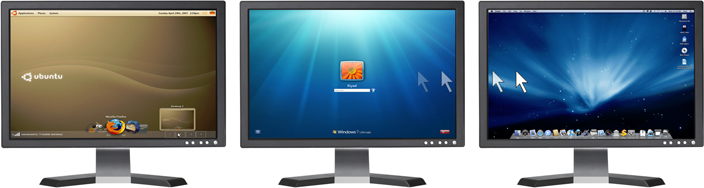
\includegraphics[height=1.6cm]{fig/PCs.png}\pause
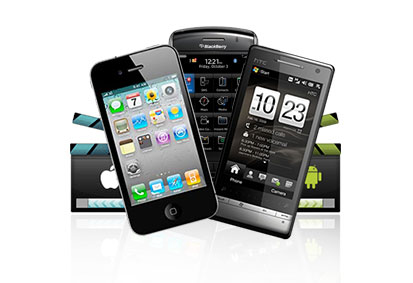
\includegraphics[height=1.0cm]{fig/mobile-bc.png}\pause
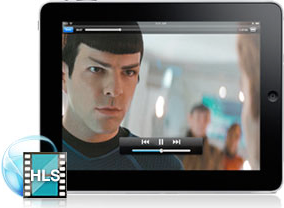
\includegraphics[height=1.1cm]{fig/streaming-bc.png}\pause

\includegraphics[height=1.6cm]{fig/video_quality-bc.png} \pause
\item 多种屏幕大小\\ %\pause
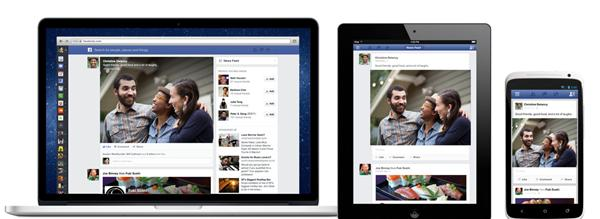
\includegraphics[height=1.2cm]{fig/screen_sizes.jpg}\pause
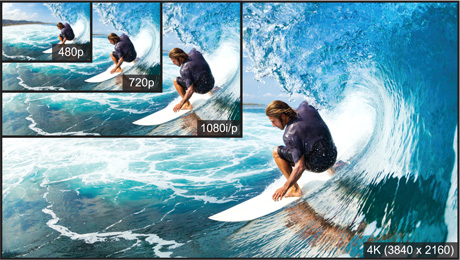
\includegraphics[height=2.2cm]{fig/480_to_4KVideo.jpg}\pause
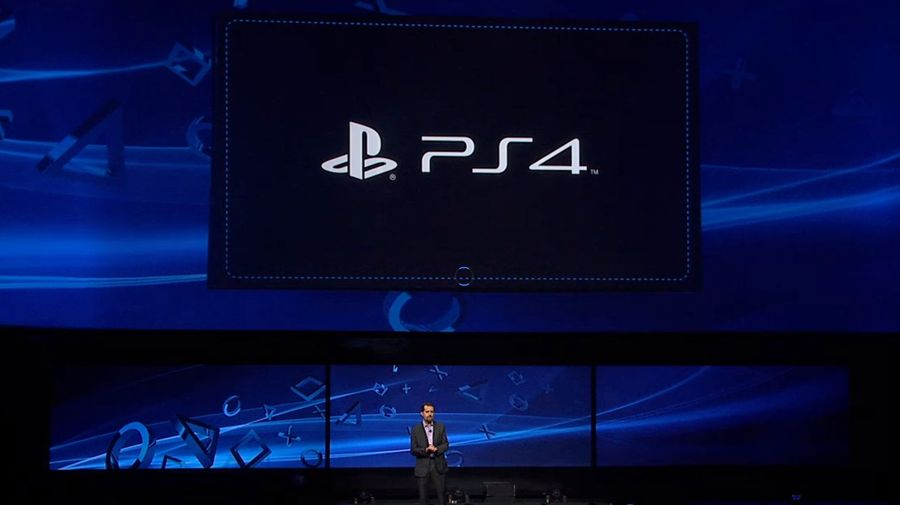
\includegraphics[height=2.2cm]{fig/4k_video.jpg} \pause
\end{itemize}
\end{frame}
\begin{frame}{多屏时代的挑战} 
\begin{itemize}
\item 多种码率\\ %\pause
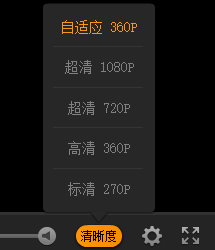
\includegraphics[height=1.9cm]{fig/bitrate_tencent.png}\hspace*{0.4cm}\pause
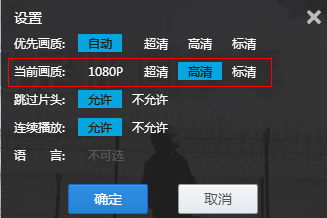
\includegraphics[height=1.9cm]{fig/bitrate_youku.png}\hspace*{0.4cm}\pause
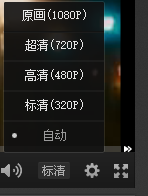
\includegraphics[height=1.9cm]{fig/bitrate_sohu.png}\hspace*{0.4cm}\pause
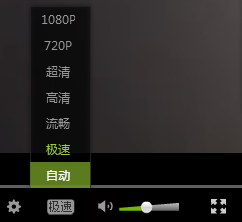
\includegraphics[height=1.9cm]{fig/bitrate_qiyi.png}\pause   
\item 多种解码能力\\ %\pause
%!!!!!!m目前支持HEVC的手机:Galaxy S4, LG G2, Nexus5, 小米3联通版, 红米1S/2... 
%\begin{table}
{\scriptsize
\begin{center}
\begin{tabular}{l|llll} %\toprule
\hline
联发科芯片& MT6572 & MT6582 & MT6588 & MT6592 \\ %\midrule
\hline
Display  & 960$\times$540P & 1280$\times$720P & 1920$\times$1280P & 1920$\times$1280P \\
H.264 Decode   & 720P@30fps & 1080P@30fps  & 1080P@30fps  & 1080P@30fps \\ 
HEVC Decode   &  N/A &  N/A  & 720P@30fps  & 720P@30fps \\ 
\hline
%\bottomrule
\end{tabular}
}
\end{center}
%\end{table}
\end{itemize}
\end{frame}
\begin{frame}{多屏时代的挑战} 
\begin{itemize}
\item 不同封装容器支持\\ %\pause
mp4, mkv, avi, flv, wmv, rmvb, webm, mpeg-ts... \pause
\item 不同编码标准支持\\ \pause
H.264(AVC), H.265(HEVC), VC-1, AVS, VP8/9, RealVideo...
\pause
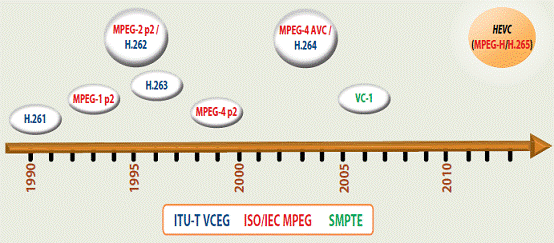
\includegraphics[height=3.5cm]{fig/encoding_standards.png}\pause
\end{itemize}
\end{frame}
\begin{frame}{多屏时代的挑战} 
\begin{itemize}
\item 巨头角力\\ %\pause
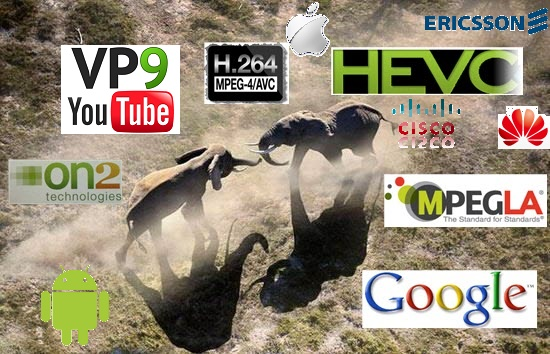
\includegraphics[height=5cm]{fig/competition.jpg}\pause
\end{itemize}
\end{frame}
\begin{frame}{幸运的是,}
\pause
绝大多数设备都支持:
\pause
\begin{itemize}
\item 编码标准\\ \pause
\small{H.264/AVC (ISO/IEC 14496-10;  ITU-T H.264; MPEG-4 Part 10).}
\item 封装容器\\ \pause
\small{MP4 (ISO/IEC 14496-14; MPEG-4 Part 14).}
\end{itemize}
\pause

$ Source \rightarrow [~ MP4, H.264, AAC ~]\left\{
\begin{array}{ccc}
version_1       &      & {(x_1 ~ kbps)}\\
version_2     &      & {(x_2 ~ kbps)}\\
\vdots     &      & {\vdots}\\
version_n       &      & {(x_n ~ kbps)}
\end{array} \right. $
\end{frame}
\begin{frame}{但是,}
\pause
\begin{itemize}
\item 媒体转码是件极其消耗计算资源的工作\\ %\pause
	尤其视频编码,对于目前常见的支持SSE4指令集的x86/x64 CPU的机器:
	\begin{itemize}
	\item  编码H.264视频需要耗费播放时长的1/3到2/3
	\item  编码H.265视频需要耗费播放时长的30+倍
	\item  单个CPU核通常最多可跑1--2个编码任务
	\end{itemize}
\item 媒体文件大,再加上多码率副本,极其消耗存储
\item 潜在的带宽消耗
\end{itemize}
\end{frame}

\begin{frame}{以往的解决:并行与分布式(Criteria)}
\begin{itemize}
\item 单机内\\
	\begin{itemize}
	\item 宏块组/帧级并行
	\item SMP/NUMA友好
	\item SIMD (SSE2, SSE4, AVX...)
	\item CPU $\rightarrow$ GPU (QuickSync, CUDA, APP...)
	\end{itemize}
\item 分布式转码
	\begin{itemize}
		\item 分布式存储
		\item 网络传输
		\item 资源分配、任务调度
	\end{itemize}
\item Enough???
\end{itemize}
\end{frame}

% -----------------------------------------------------------------------------
\section{从Cloud Transcoder到TranscX}
\subsection{前腾讯研究院Cloud Transcoder}
\begin{frame}{前腾讯研究院Cloud Transcoder}
\textbf{Done 2011-. Gale Huang et al. Cloud transcoder: bridging the format and resolution gap between internet videos and mobile devices. ACM NOSSDAV 2012.}\\\pause
\begin{center}
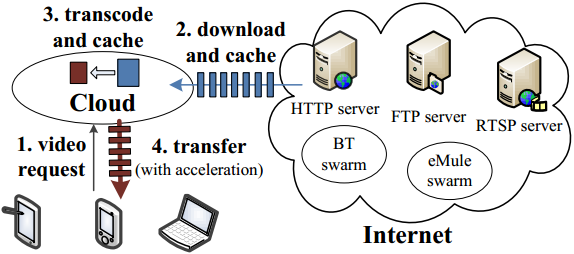
\includegraphics[height=2.8cm]{fig/clouder-transcoder_principle.png}\\\pause

\includegraphics[scale=0.36]{fig/cloud_transcoder_nossdav_affiliation.png}
\end{center}
\end{frame}

\begin{frame}
\begin{center}
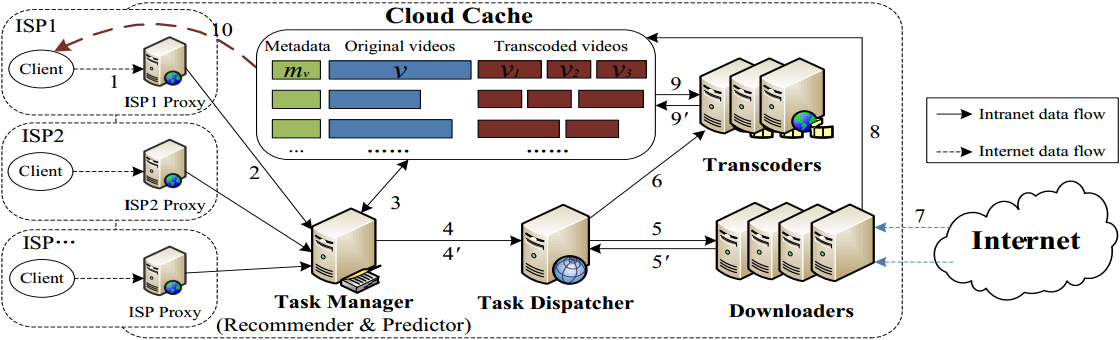
\includegraphics[width=11.5cm]{fig/cloud-transcoder_arch.png}
\end{center}
\end{frame}
\begin{frame}
\begin{center}
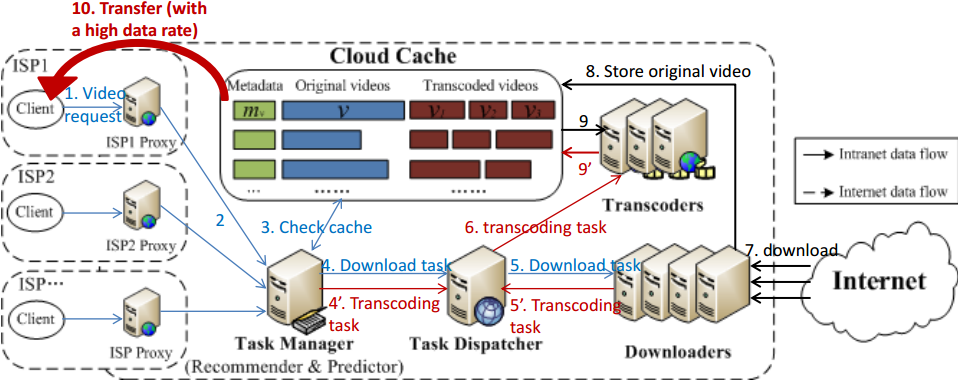
\includegraphics[width=11.5cm]{fig/cloud-transcoder_arch_details.png}
\end{center}
\end{frame}
\begin{frame}
\begin{center}
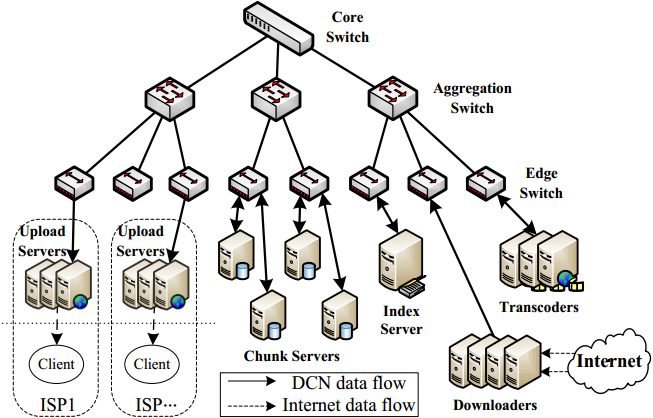
\includegraphics[width=10cm]{fig/cloud-cache_hardware.png}
\end{center}
\end{frame}
\begin{frame}{评价}
\begin{itemize}
	\item 整体上是个设计优秀的系统
	\item 但还存在一些问题:
	\begin{itemize}
		\item 下载、转码、任务分发、任务管理都需要专门的机器资源
		\item 下载后,数据还需要再次传输到相应的转码机器
		\item 做切片的开销
		\item 划分的各模块,增加了部署复杂性,限制了可扩展性
		\item 存储部分依赖NFS,不能支持海量的媒体资源
		\item 转码完成后,分发是个问题
	\end{itemize}
\end{itemize}
\end{frame}

\subsection{架平流媒体TranscX}
\begin{frame}{架平流媒体TranscX}
TranscX: 
\begin{itemize}
	\item Transcoding eXpress/eXperience/eXtreme...; transc(x)
\end{itemize}
\pause
\begin{center}
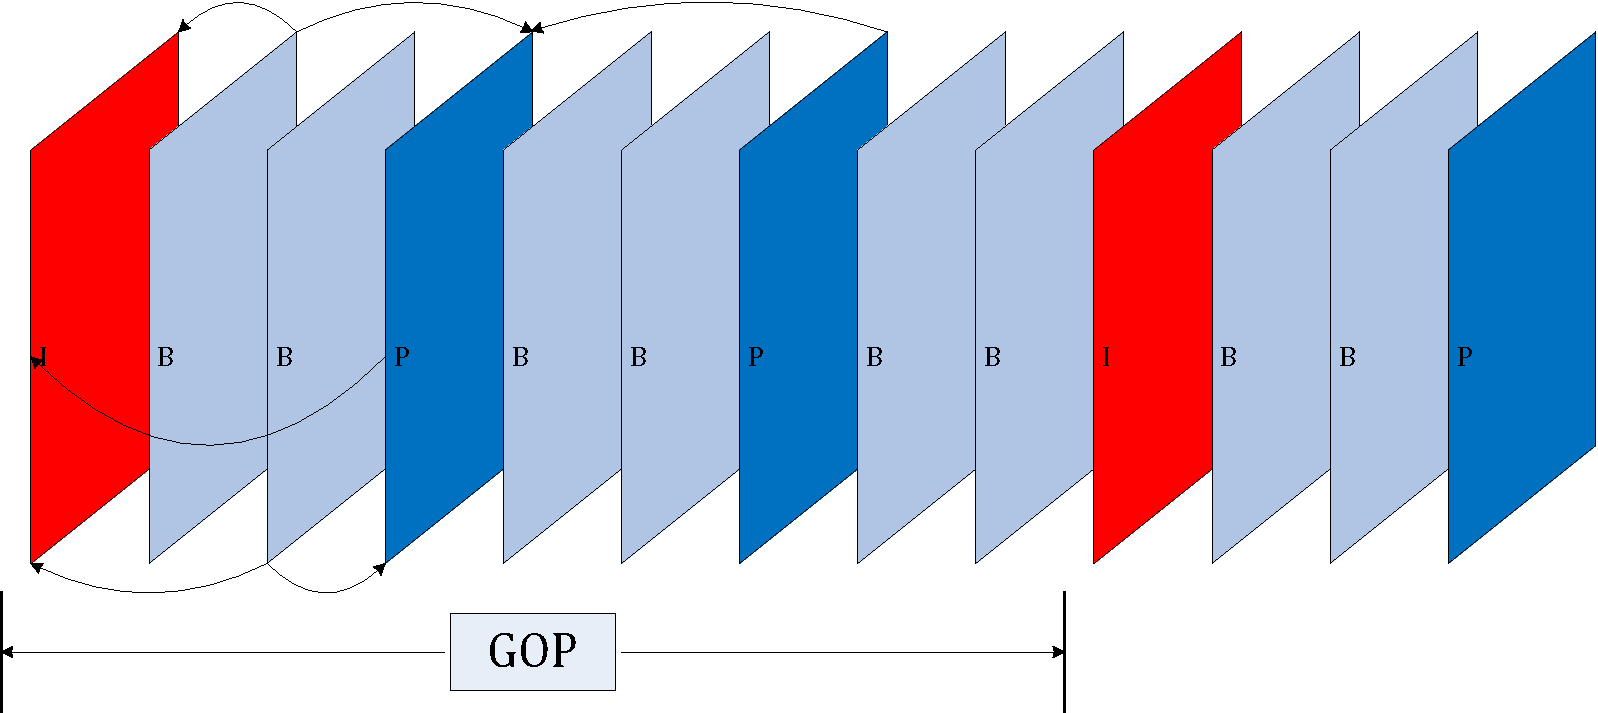
\includegraphics[scale=0.20]{fig/GOP.pdf}
\end{center}
\begin{itemize}
\item GOP级的并行,不需要真正“切割”\\
Media head parsing, <begin\_time, end\_time> or GOP\_id $\rightarrow$ <start\_offset, size>
\end{itemize}
\end{frame}

\begin{frame}
\begin{itemize}
\item I\\

\includegraphics[scale=0.40]{fig/cjk1.jpg}
\end{itemize}
\end{frame}
\begin{frame}
\begin{itemize}
\item B\\

\includegraphics[scale=0.40]{fig/cjk2.jpg}
\end{itemize}
\end{frame}
\begin{frame}
\begin{itemize}
\item B\\
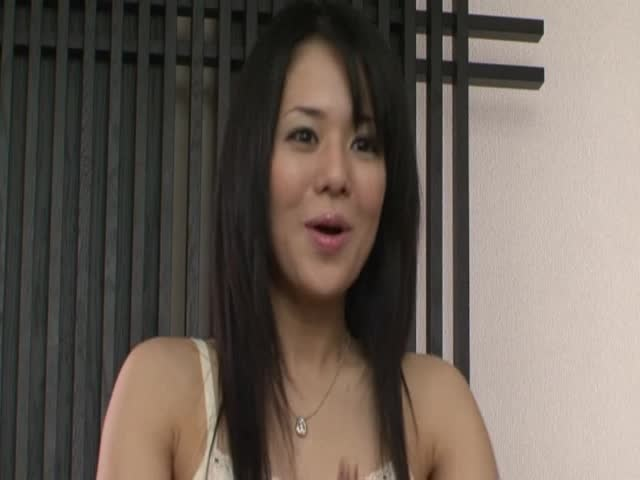
\includegraphics[scale=0.40]{fig/cjk3.jpg}
\end{itemize}
\end{frame}
\begin{frame}
\begin{itemize}
\item P\\

\includegraphics[scale=0.40]{fig/cjk4.jpg}
\end{itemize}
\end{frame}
\begin{frame}
\begin{itemize}
\item I: IDR\\

\includegraphics[scale=0.40]{fig/bfj1.jpg}
\end{itemize}
\end{frame}
\begin{frame}
\begin{itemize}
\item B\\

\includegraphics[scale=0.40]{fig/bfj2.jpg}
\end{itemize}
\end{frame}
\begin{frame}
\begin{itemize}
\item B...\\

\includegraphics[scale=0.40]{fig/bfj3.jpg}
\end{itemize}
\end{frame}

\begin{frame}
\begin{center}
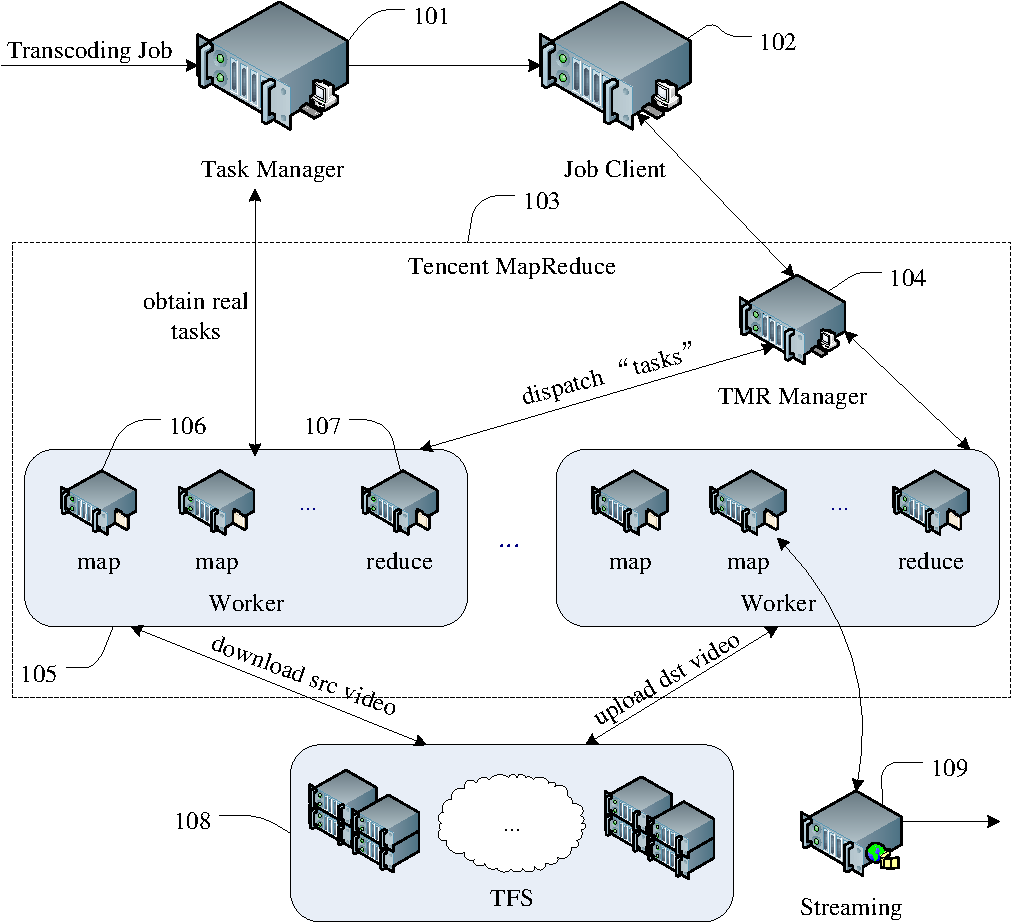
\includegraphics[height=6.4cm]{fig/TranscX.pdf}
\end{center}
\end{frame}
\begin{frame}
\begin{center}
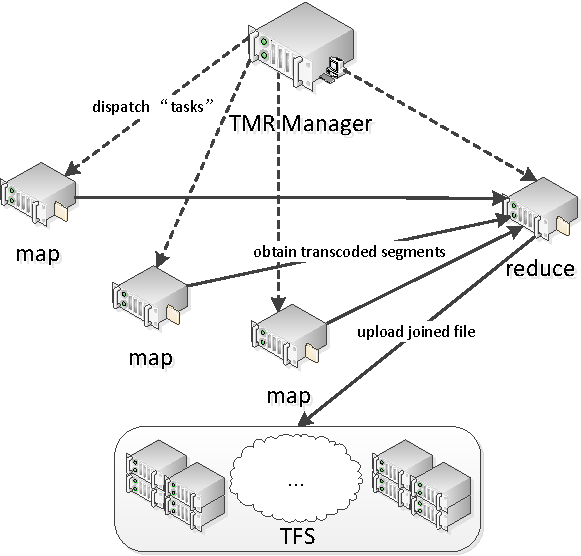
\includegraphics[height=6.2cm]{fig/TranscX_detail.pdf}
\end{center}
\end{frame}

\begin{frame}
\begin{itemize}
\item 避免影响存储集群的现网服务?\\
Job/Map/Thread三级精确控制,CPU \& I/O limitation
\item 效率高在哪里?\\
转码工作在存储机器上完成,减少数据传输,接近本地计算--计算向存储迁移
\item 架构好在哪里?\\
MapReduce(Typhoon)? TFS/CFS? Protocol? 
\item 复用存储服务器的空闲计算资源,减少碳排放(绿色计算)
\item WeChat, Qzone, Weishi? 
\item 对DASH和实时在线直播的支持
\end{itemize}
\end{frame}

\section{DASH与稳定婚姻}
\subsection{DASH}
\begin{frame}{Why DASH?}
%DASH: Dynamic Adaptive Streaming over HTTP.
\pause
\begin{itemize}
\item 庞大的文件头,导致在线播放时较大的initial/VCR delay
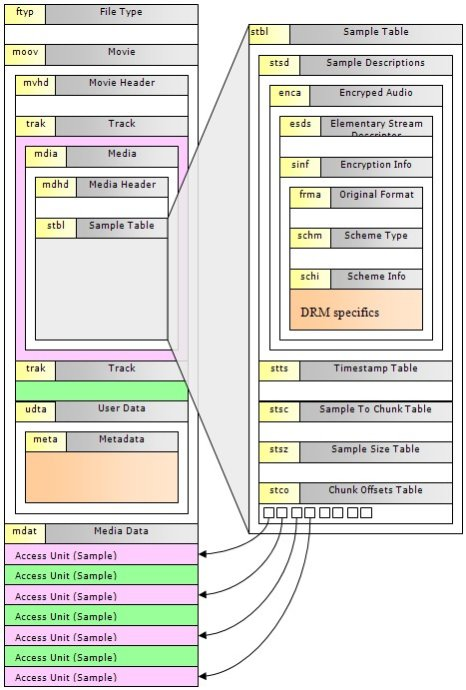
\includegraphics[height=4cm]{fig/MP4_boxes_detail.jpg}
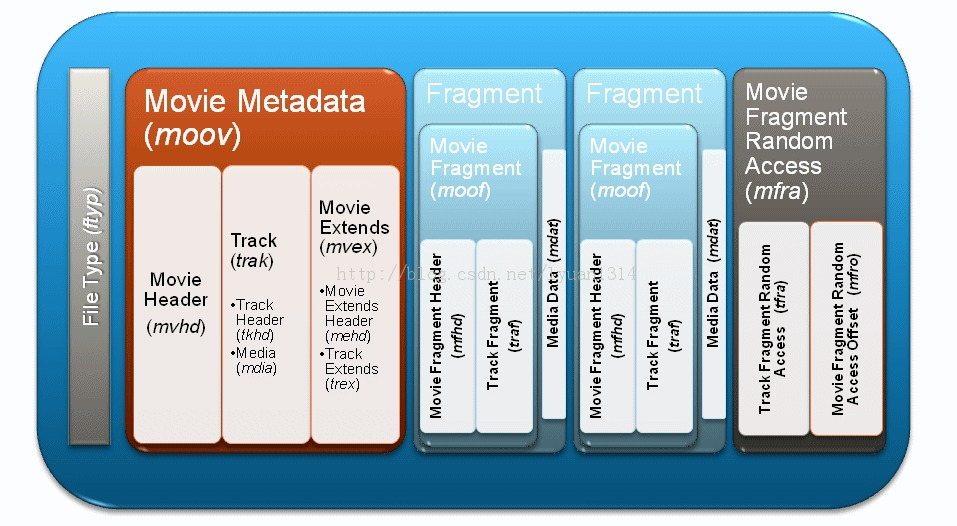
\includegraphics[height=4cm]{fig/fragmented_mp4.jpg}
\end{itemize}
\end{frame}
\begin{frame}
\begin{itemize}
\item 二次缓冲频繁 due to varying download speed \\
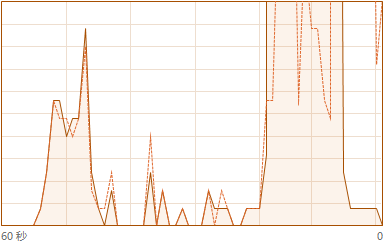
\includegraphics[height=5.4cm]{fig/download_speed.png}
\end{itemize}
\end{frame}
\begin{frame}{DASH}
DASH: Dynamic Adaptive Streaming over HTTP. \\
几种DASH标准:
\pause
\begin{itemize}
\item Apple HLS (HTTP Live Streaming) 2009
\item Microsoft HSS (HTTP Smooth Streaming) 2010
\item Adobe HDS (HTTP Dynamic Streaming) 2010
\item MPEG-DASH (ISO/IEC 23009-1) 2012
\end{itemize}
\end{frame}
\begin{frame}{Apple HLS}
\begin{itemize}
\item Architecture
\begin{center}
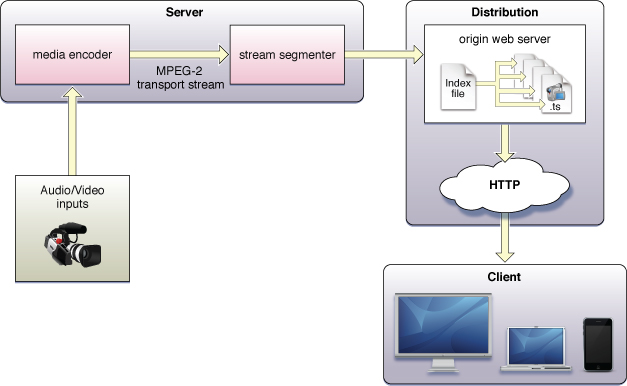
\includegraphics[height=4.5cm]{fig/hls_arch.jpg}
\end{center}
\end{itemize}
\end{frame}
\begin{frame}{Apple HLS}
\begin{itemize}
\item Segment Indexing
\begin{center}
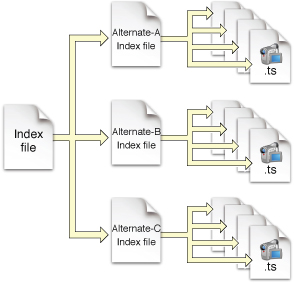
\includegraphics[height=4.5cm]{fig/hls_indexing.jpg}
\end{center}
\end{itemize}
\end{frame}

\begin{frame}{MPEG-DASH}
\begin{itemize}
\item Architecture
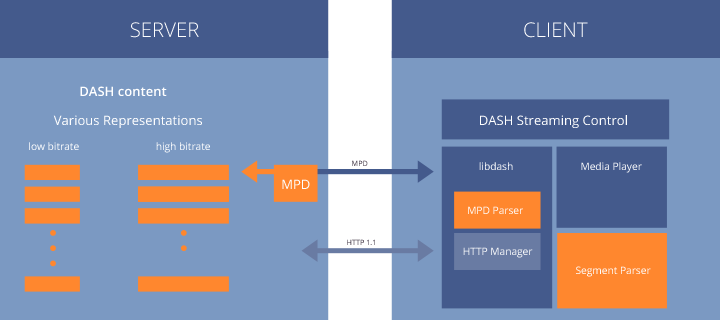
\includegraphics[height=4.5cm]{fig/MPEG-DASH_arch.png}
\end{itemize}
\end{frame}
\begin{frame}{MPEG-DASH}
\begin{itemize}
\item Data Model
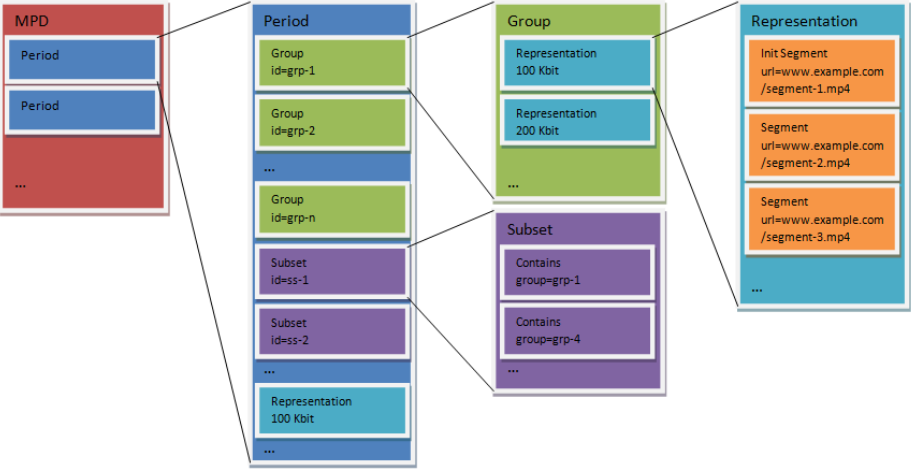
\includegraphics[height=4.5cm]{fig/mpeg-dash_data_model.png}
\end{itemize}
\end{frame}
\begin{frame}{MPEG-DASH}
\begin{itemize}
\item Segment Indexing
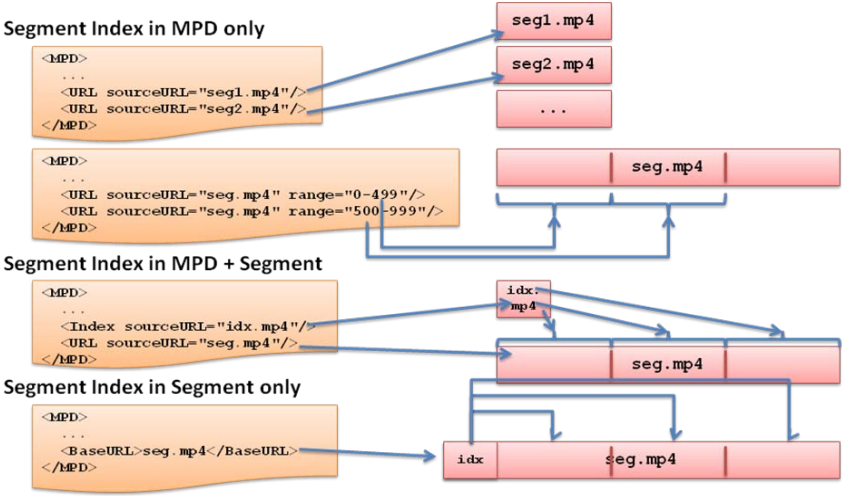
\includegraphics[height=5cm]{fig/mpeg-dash_indexing.png}
\end{itemize}
\end{frame}

\begin{frame}{原有系统怎么完成DASH改造?架平流媒体经验}
\begin{itemize}
\item 转封装 vs 转编码?\\
尽量只转封装,不转编码;实时、按需转封装/转码
\item 并发I/O流少的问题?使用/自写的协议?
	\begin{description}
	\item[tmpfs] 最简单、方便,对Cache管理要求不强的场合
	\item[in\_mem] in memory, 进程内的编解码I/O
	\item[shm\_mem] shared memory, 多进程的编解码I/O,可自定义Cache管理、淘汰算法
	\item[AVIOContext] FFMPEG built-in
	\item[async\_http] 适用直播,数据到达不可预期 %read frame --> decode --> encode
\end{description}
\item FPGA HEVC Encoding (proposed)
\end{itemize}
\end{frame}

\subsection{稳定匹配}
\begin{frame}{新的问题}
DASH和WeChat, Weishi, Qzone等社交UGC视频转码中存在的问题:\pause
\begin{itemize}
\item 视频长度较短\\
一般仅一个到若干个GOP,MapReduce时仅需要一个Mapper,不需要Reducer
\item MapReduce任务调度延时较大,甚至超播放时长\\
可通过批量提交或LXC, Docker守护进程的实时In-memory MapReduce来缓解,但非根本解决之道
\item 大部分视频的未来访问少于X次\\
还有必要全码率转码+全量分发么?
\end{itemize}
\end{frame}
\begin{frame}{大数据分析,得出结论:}
\begin{itemize}
	\item 对数千台后台服务器连续一周运行状态的测量:\\
		\begin{itemize}
		\item 不仅DC,OC的多数服务器大部分时间CPU负载也较低\\
		甚至包括某些HTTP服务器
		\item 多数服务器的CPU负载基本不会出现突变\\
		CPU负载随时间相对平稳,但不同地区的平均负载存在差异
		\end{itemize}
	\item 对应时间所有用户访问和调度情况的测量:\\
		\begin{itemize}
		\item 用户对CDN的region选择存在偏好\\
		由于网络拓扑关系,用户去不同的CDN边缘节点下载的速率各不相同,而目前的调度算法,至少能得到一个次优解
		\item 不同地区用户对码率存在偏好\\
		在前面次优解的前提下,不同地区得到平均服务质量有差异
	\end{itemize}
\end{itemize}
\end{frame}
\begin{frame}{带宽和CPU使用率示例}
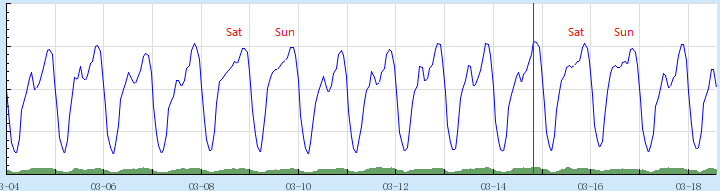
\includegraphics[height=2.4cm]{fig/bandwidth.png}\\
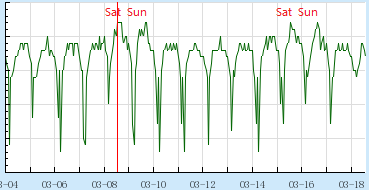
\includegraphics[height=3.2cm]{fig/cpu_usage.png}
\end{frame}
\begin{frame}{启发}
\begin{itemize}
\item CDN的大部分服务器是否也可用来做转码?\\
\item 是否可以按需转码,按需分发?\\
on-line, on-the-fly, on-demand?
\item 当前CDN节点实在是没有所需码率片段时...\\
是否可以给一个不高于所需码率的最高码率副本来替代?
\end{itemize}
\end{frame}

\begin{frame}{优化问题}
\begin{itemize}
\item 用户重定向\\
用户当前请求应该被调度到哪个CDN节点来服务?资源应尽量在哪儿转码?服务器负载、带宽利用、用户体验,哪个更重要?
\item 哪些资源的哪些片段最需要被转码\\
用户最需要的,能尽量让用户得到最大码率的,当前副本最少的?消耗服务器计算资源少的(节能/碳环保)?
\item 转码后的片段应当怎样在CDN云中分发\\
怎样定义分发代价?怎样让代价最小?怎样尽可能不超出购买带宽量?
\end{itemize}
\end{frame}
\begin{frame}{我们的启发式算法}
\begin{itemize}
\item 联合考虑转码和分发,再多阶段优化
\item 三个扩展的0-1背包问题
\item 用户--服务器--码率副本? ---调度/匹配?\pause
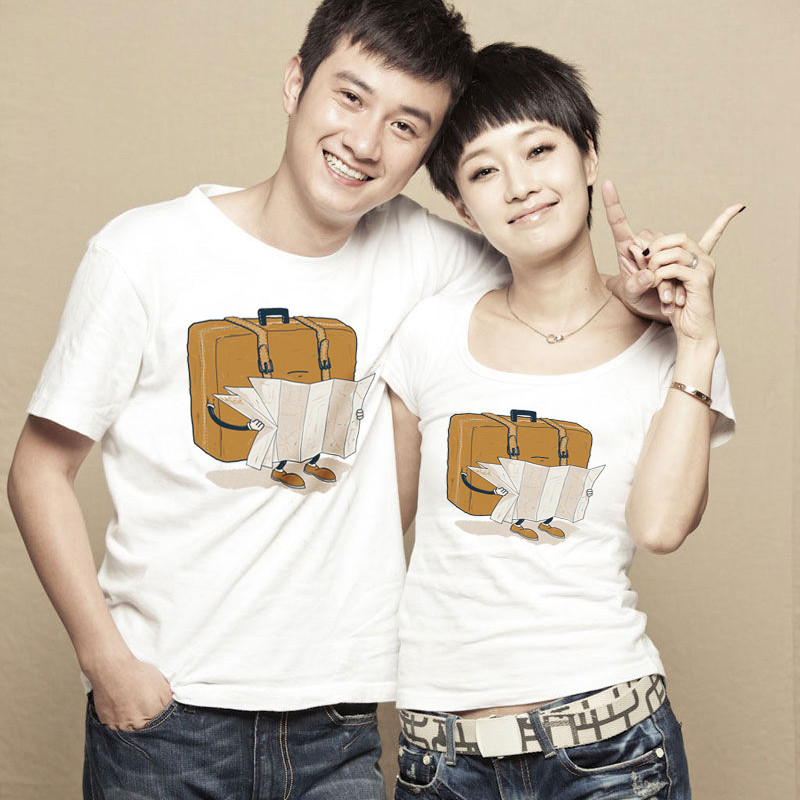
\includegraphics[height=2.7cm]{fig/wenzhang_mayili.jpg}\pause
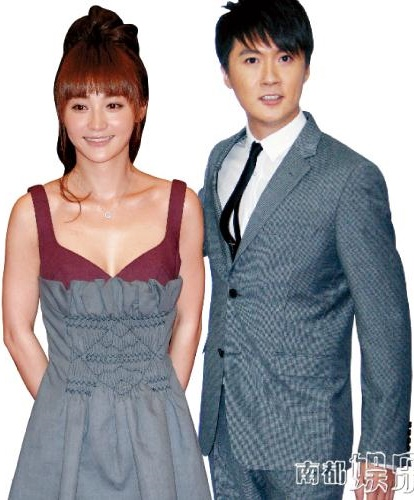
\includegraphics[height=2.7cm]{fig/yaodi_chishuai1.jpg}\pause

\includegraphics[height=2.7cm]{fig/yaodi_chishuai.jpg}\pause
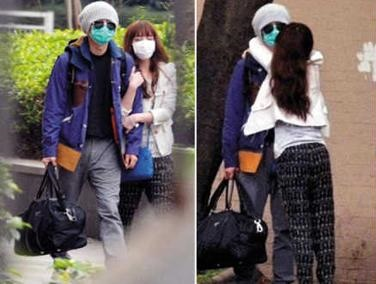
\includegraphics[height=2.7cm]{fig/wenzhang_yaodi.jpg}
\end{itemize}
\end{frame}
\begin{frame}{我们的启发式算法}
\begin{itemize}
\item 启发式规则和稳定匹配(婚姻)结合
	\begin{itemize}
		\item 启发式:设计出贪心规则给出NP难问题的近似最优解
		\item 稳定匹配:扩展的稳定婚姻问题\\
			\begin{itemize}
					\item 女追男---尽量利于女神\\
						女:用户;男:CDN边缘节点
					\item 男方具有多容量
					\item 稳定性、最优性与帕累托效率
			\end{itemize}
	\end{itemize}
\end{itemize}
\end{frame}

\begin{frame}{算法应用}
准备与预测框架\\
\begin{itemize}
\item 用户对所有CDN边缘节点的偏好\\
过去的测速数据$\rightarrow$Rank用户对所有CDN边缘节点的偏好
\item 每段视频未来一段时间的访问频率\\
过去访问频次\&幂律分布\&指数衰减\&传播模式$\rightarrow$未来一段时间所有有可能有访问的视频的访问频次
\item 未来一小段时间服务器的期望空间计算资源\\
工作日/周末自回归模型\&短时线性回归$\rightarrow$未来一段时间每个OC节点服务器的期望CPU负载
\end{itemize}
\end{frame}
\begin{frame}{整体架构与“女追男”模型}
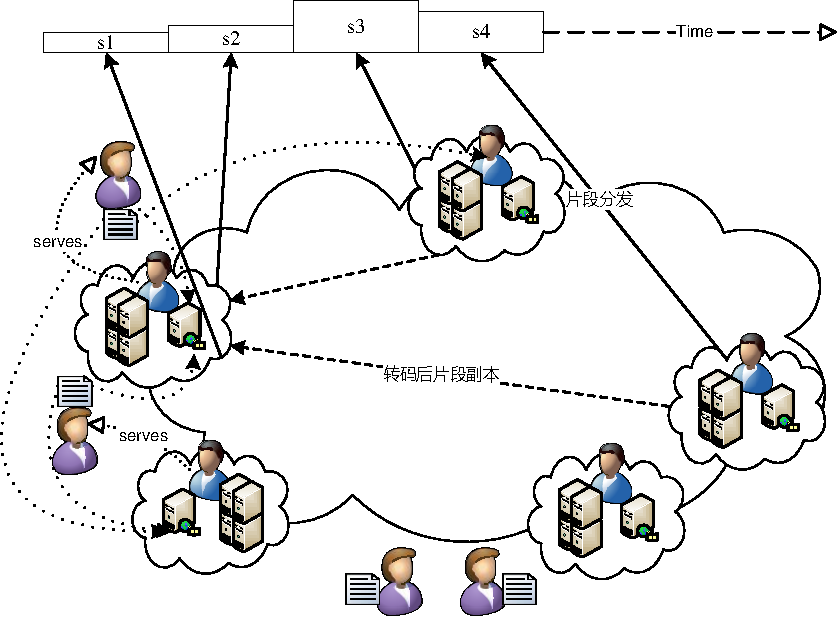
\includegraphics[height=5.6cm]{fig/transcoding_delivery.pdf}
\end{frame}
\begin{frame}{至关重要:Satisfying Women}
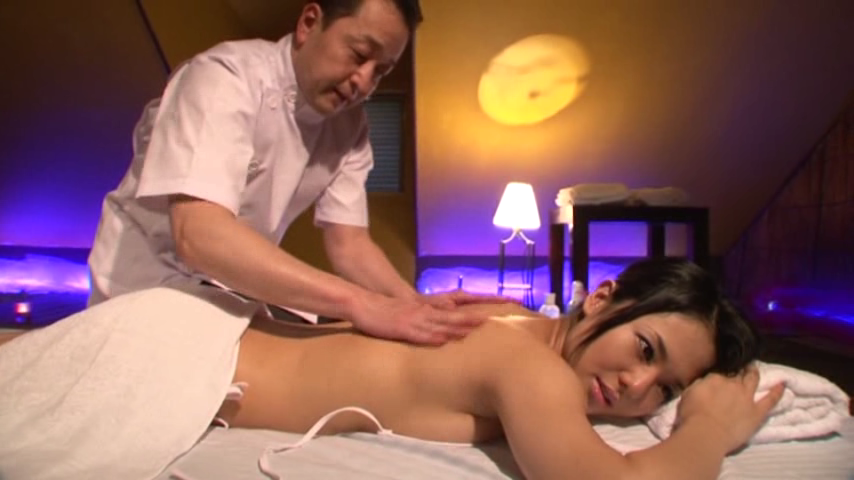
\includegraphics[height=5.6cm]{fig/massage2.png}
\end{frame}
\begin{frame}{效果}
\begin{itemize}
\item 44.8\%的用户会享受更高码率的版本\\
	相比传统服务器负载均衡的算法
\item 4.5倍的用户享受到最高的可能码率\\
	%相比传统服务器负载均衡的算法
\item 减少42.2\%接受和当前带宽不匹配码率的可能\\
	相比传统FIFO(先来先服务)的算法
\item 减少约80\%的转码计算资源消耗\\
	对于微视、腾讯视频这种4码率副本的场景。码率副本数越高,效果越明显。(Qzone两码率副本场合,减少约40\%)
\item 副本传输的带宽不随分段数显著增长\\
	事实上,当分段数$n$足够大后,随$n$几乎不变了。
\end{itemize}
\end{frame}
\begin{frame}{Publications}
\begin{center}

\includegraphics[width=10cm]{fig/infocom.jpg}\\\pause
...alanzhuang... Joint Online Transcoding and Geo-distributed Delivery for Dynamic Adaptive Streaming. IEEE Transactions on Parallel and Distributed Systems (TPDS). 2014. (will appear)\\\pause
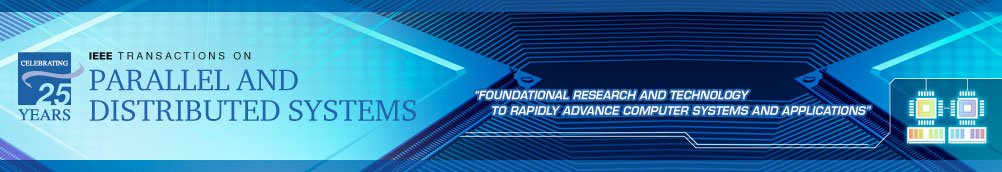
\includegraphics[width=10cm]{fig/tpds_25yr.jpg}\\\pause
\end{center}
\end{frame}

\section{Future Vision \& Others}
\subsection{和一些新技术的结合}
\begin{frame}{和一些新技术的结合}
\begin{itemize}
\item WebRTC\\
Client-end caching \& delivery \& broadcasting
\item HTML5 WebSocket, HTTP 2.0\\
会话保持,多流传输
\item Social Could TV\\
\item HEVC, SVC, MVC, NC\\
编码、多副本多版本机制、多视角、传输
\end{itemize}
\end{frame}
\begin{frame}{友商的行动--新闻报道}

\includegraphics[height=1.0cm]{fig/rmw_logo.jpg}

\includegraphics[height=1.0cm]{fig/xinhua_logo.jpg}

\includegraphics[height=1.0cm]{fig/huanqiu_logo.jpg}

\includegraphics[height=1.0cm]{fig/taobao_logo.jpg}\\\pause
\small{
继空调之后,电视台成为XX云计算的下一个大数据重塑目标。2014年3月20日下午,XX云宣布...打造中国最大的全媒体云计算平台。...在一周内,帮助传统电视台变成多屏网络电视台,支持电脑网站、手机APP、电视机全终端流畅播放,...

XX云是中国罕有可以将5000台计算机合成一台“超级计算机”的云计算平台,将为全国广播电视媒体提供超级计算、高速存储和网络连接能力,满足其海量视频内容的处理和传播需求。合作伙伴新奥特则负责开发基于云平台的全媒体播控系统,包括采集收录、快编转码、存储管理、多终端视频发布、收视研究等。...,其中包括中央电视台,北京、江苏、浙江、湖南卫视等多家强势电视媒体。
}
\end{frame}
\begin{frame}
\begin{center}
\includegraphics[height=7.6cm]{fig/tengyun.jpg}
\end{center}
\end{frame}
\subsection{Acknowledgment}
\begin{frame}{Acknowledgment}
本slide中部分内容源自与以下人员的协作/交流:
\begin{itemize}
\item 架平流媒体\\
Leon, Devin, Guita, Wood, Kernel, Chris
\item Tsinghua-Tencent Joint Lab.\\ 
Zhi Wang
\item SNG社交平台部\\
Stone Huang, Scorpion Xu, Rizen Guo
\item Nanyang Technological University\\
Young Wen
\end{itemize}
\end{frame}
\begin{frame}{Q\&A?}
\begin{center}
\includegraphics[height=6.0cm]{fig/tengyun.jpg}
\end{center}
\end{frame}
% -----------------------------------------------------------------------------
\end{document}
